\documentclass[11pt,a4paper]{article}
\usepackage[margin=2.4cm]{geometry}
\usepackage[utf8]{inputenc}
\usepackage[T1]{fontenc}
\usepackage{mathptmx}
\usepackage{amsmath,amssymb}
\usepackage{booktabs}
\usepackage{graphicx}
\usepackage{xcolor}
\usepackage[round,authoryear]{natbib}
\usepackage[colorlinks=true,citecolor=blue!50!black,linkcolor=blue!50!black,urlcolor=blue!50!black]{hyperref}
\usepackage{caption}
\captionsetup{font=small,labelfont=bf}

\title{\textbf{When Does External Retrieval Help Video Captioning? Evidence Budgets in a Million-Clip Memory}}
\author{[Author Name 1]$^{1}$, [Author Name 2]$^{1}$, \ldots, [Corresponding Author Name]$^{1,*}$\\[4pt]
\small $^{1}$[Department, Institution, City, Country --- TO BE COMPLETED BY AUTHORS]\\
\small $^{*}$Corresponding author: \texttt{[email@institution.edu --- TO BE COMPLETED BY AUTHORS]}}
\date{}
\begin{document}
\maketitle

\begin{abstract}
Expanding an external retrieval memory gives a video captioner access to closer candidate descriptions, yet improved retrieval access does not ensure better generated captions. We investigate this gap in a fixed retrieval-augmented video captioning framework paired with six nested VideoUFO external memories spanning 10,000 to 1,091,712 clips. Across the nested corpus endpoints, selected top-one X-CLIP similarity rises reliably while fixed-budget generation utility exhibits no consistent improvement. On both MSR-VTT and MSVD test benchmarks, smaller joint text--visual evidence budgets consistently outperform seven retrieved pairs. Because positive-budget sweeps alone cannot determine whether any external example earns its place in the prompt, we conducted two prespecified interventions on the previously analyzed MSR-VTT benchmark using source-cluster bootstrap and sign-flip inference with Holm adjustment. Relative to a matched zero-evidence control that retains the full prompt scaffold and cross-gating fusion pathway (A0, 69.81 CIDEr), supplying one external caption--clip pair improved CIDEr by +1.40 points (95\% pointwise source-cluster CI [+0.45, +2.36]; family Holm \emph{p} = .0066; five-test Holm \emph{p} = .0165), whereas seven pairs reduced CIDEr by $-$1.54 points ([$-$2.94, $-$0.18]; family Holm \emph{p} = .0271; five-test Holm \emph{p} = .0813). In a second intervention holding all three retrieved visual tensors and intermediate fused representations strictly identical per query (n = 2,618), appending four higher- or lower-similarity captions shifted CIDEr by $-$1.27 ([$-$2.34, $-$0.20]; family Holm \emph{p} = .0573) and $-$1.13 points ([$-$2.15, $-$0.14]; family Holm \emph{p} = .0612), with an inconclusive direct contrast between similarity bands ($-$0.14, [$-$1.05, +0.80]; \emph{p} = .7698). None of the five planned intervals cleared the prespecified $\pm$1.0-point practical significance margin. Taken together, a minimal external evidence budget delivers measurable net benefit over zero external evidence in this fixed system, whereas neither retrieval similarity alone nor an unconfirmed general text-overload mechanism explains performance at larger budgets.
\end{abstract}
\noindent\textbf{Keywords:} Video captioning; Retrieval-augmented generation; External multimodal memory; Evidence budgeting; Paired source-cluster evaluation

\section{Introduction}
Retrieval-augmented video captioning aims to ground natural-language generation in related examples drawn from an auxiliary memory. In practice, however, visual similarity between a query video and a retrieved clip is an imperfect proxy for caption utility. A candidate clip can resemble the query scene while depicting a different action, and concatenating multiple individually plausible descriptions into one prompt can alter how the language decoder weighs visual against textual cues. Scaling the searchable corpus changes what evidence can be retrieved, whereas changing the evidence budget alters how much retrieved text and visual context enters the generator. Diagnosing external retrieval therefore requires separating candidate availability from downstream caption quality and testing whether retrieved examples actually outperform the same system operating without external evidence.

Recent work by \\citet{Fang2026EVCap} introduced a retrieval-augmented video captioner built on Video-LLaMA and Vicuna-7B that combines X-CLIP caption retrieval, unsupervised quality-aware reranking, and similarity-weighted cross-gating fusion over corresponding video features. Evaluating in-domain training memories on MSR-VTT and MSVD, Fang et al. showed that the number of retained examples affects captioning accuracy, adopting seven examples for MSR-VTT (peaking at \emph{k} = 7 in their sweep from one to ten) and three for MSVD. Because their architecture is already established and sensitivity to \emph{k} is known in-domain, repeating a budget sweep on a new corpus does not by itself constitute a distinct scientific contribution.

Instead, we hold Fang et al.'s captioning architecture and checkpoints fixed and ask a more targeted diagnostic question: how does evidence utility behave when a compact in-domain training memory is replaced by a million-clip external collection of machine-described videos? We organize this investigation around three linked research questions:

\begin{itemize}
\item \textbf{RQ1 (Candidate access versus generation utility):} When an external video memory expands from 10,000 to 1,091,712 clips, do gains in retrieval similarity and candidate turnover translate into consistent improvements in fixed-budget caption quality?
\item \textbf{RQ2 (Net retrieval utility):} Given that smaller joint budgets outperform larger ones on external retrieval, does a small external evidence budget actually yield a net gain relative to the exact same fusion-enabled system receiving zero external evidence, and can larger budgets push net utility below zero?
\item \textbf{RQ3 (Selection headroom and textual attribution):} To what extent do candidate selection within a fixed top-20 pool and textual expansion under verified identical retrieved visual representations account for the budget response?
\end{itemize}
Answering RQ2 and RQ3 resolves two ambiguities that positive-budget comparisons cannot address on their own. First, observing that one retrieved example outscores seven does not tell us whether one example helps or whether all external budgets degrade a captioner relative to an empty-evidence baseline. Testing net utility cleanly requires retaining the trained checkpoint, prompt scaffold, and cross-gating fusion module while setting external inputs to zero. Second, because joint budgets couple retrieved captions with their corresponding clip features, a drop from three to seven examples could arise from textual prompt expansion, altered visual aggregation, or both. Isolating textual extensions requires verifying per-query identity of the actual retrieved visual tensors and intermediate fused representations before comparing appended caption sets.

Following this progression---from candidate access, to matched net retrieval utility, to controlled evidence extension and attribution---this study makes three contributions:

\begin{enumerate}
\item \textbf{Nested million-clip scale and cross-benchmark budget characterization:} Across six nested VideoUFO memories (10K to 1.09M clips) and two retrieval orderings, we show that substantial increases in selected X-CLIP similarity and candidate replacement do not produce consistent fixed-budget CIDEr gains, while smaller joint budgets reliably outperform seven examples on both MSR-VTT and MSVD under their inherited checkpoints.
\item \textbf{Matched zero-evidence evaluation of net external utility:} Through a prespecified intervention retaining the complete fusion pathway at zero external input (Experiment A; 2,690 MSR-VTT queries across 2,004 video sources), we establish a conditional net gain of +1.40 CIDEr points for one external caption--clip pair that survives Holm correction across all five planned tests, alongside a $-$1.54-point loss at seven pairs that passes within-family adjustment but not five-test adjustment.
\item \textbf{Visual-tensor-verified textual extensions and diagnostic boundaries:} Combining repaired reference-guided Oracle diagnostics with a prespecified fixed-visual text intervention (Experiment B; 2,618 eligible queries across 1,969 sources), we quantify selection headroom in the top-20 pool and test higher- versus lower-similarity four-caption extensions under verified visual parity. Both extensions trend negatively without passing within-family Holm adjustment, and the direct similarity-band contrast is inconclusive, establishing clear evidential boundaries against overclaiming a confirmed general text-overload law.
\end{enumerate}
\section{Related Work}
\subsection{Retrieval-augmented video captioning}
Early retrieval-augmented video captioning retrieved training sentences to guide copy--generate decoding, with Open-Book Video Captioning \\citep{Zhang2021OpenBook} separately examining retrieved sentence counts, training-corpus fractions, oracle retrieval, and cross-dataset transfer. \\citet{Fang2026EVCap} coupled X-CLIP video-to-text retrieval with unsupervised caption reranking and similarity-weighted cross-gating over corresponding retrieved video features, showing in their Table 4 that MSR-VTT CIDEr rises from one to seven retained captions before declining at eight to ten, while adopting three examples for MSVD. Our study inherits their frozen captioning interface and asks how external corpus scaling, zero-evidence net utility, and visual-parity text extensions behave when retrieval shifts from in-domain training splits to a million-clip external collection.

Related retrieval mechanisms have also been developed for neighboring video-description tasks. EgoInstructor retrieves instructional third-person videos for egocentric captioning through a learned cross-view retriever and reports improvements with larger shot counts \\citep{Xu2024EgoInstructor}. In dense video captioning, CM$^2$ introduces cross-modal memory retrieval across variable feature counts and memory compositions \\citep{Kim2024CM2}, HiCM$^2$ adds hierarchical compact memory modeling with non-monotone count curves \\citep{Kim2025HiCM2}, and Sali4Vid combines saliency-aware visual reweighting with adaptive caption retrieval across event segments \\citep{Jeon2025Sali4Vid}. Unlike those jointly trained localization or cross-view architectures, our focus is single-clip captioning with a frozen multimodal generator, isolating how corpus scale, budget selection, and modality inputs behave without retraining.

\subsection{External multimodal memories and retrieval--utility divergence}
Web-scale and heterogeneous external memories have been studied prominently in image captioning and multimodal retrieval-augmented generation. SmallCap prompts a lightweight captioner with retrieved text from memories reaching 12M web captions and evaluates video transfer via a four-frame image representation \\citep{Ramos2023SmallCap}. SURf examines a million-scale image--caption datastore alongside example counts, rank-stratified distractors, and robustness training \\citep{Sun2024SURf}. VideoRAG frameworks retrieve multimodal segments to answer text queries over video collections \\citep{Jeong2025VideoRAG,Ren2026VideoRAG}. Whereas text-query VideoRAG retrieves videos for question answering and SURf trains models for selective utilization, our setting couples a query video with external caption--clip pairs through a fixed fusion interface.

Across both vision-language and text RAG, prior work has emphasized that retrieval relevance does not guarantee generation utility. RA-Transformer documented rising candidate reference overlap alongside an intermediate optimal example count in image captioning \\citep{Sarto2022RATransformer}. In text QA, SePer \\citep{Dai2025SePer} and Sufficient Context \\citep{Joren2025SufficientContext} distinguish retrieving relevant passages from using them effectively to produce accurate outputs. Large datastore scaling can yield steady gains in language modeling \\citep{Shao2024MassiveDS}, underscoring that scaling outcomes depend strongly on the task and generator interface.

\subsection{Context interference, ordering, and adaptive budgeting}
Controlled diagnostic studies in text RAG have manipulated passage ordering, relevance, and distractors, demonstrating positional sensitivity in long prompts \\citep{Liu2024LostMiddle} and distinct impacts from semantically close distractors versus random text \\citep{Cuconasu2024PowerNoise}. In multimodal question answering, MAD-RAG showed that even answer-containing retrieved text can disrupt visual attention \\citep{Zhao2026MADRAG}. Our diagnostics operate strictly at the behavioral input--output level in external video captioning; rather than probing internal attention heads, we test whether zero-evidence anchoring, visual-tensor parity, reference-guided selection, and order or removal perturbations reproduce the aggregate budget response.

Finally, query-adaptive truncation methods choose the number of retained examples per query based on retrieval score geometry. Adaptive-\emph{k} places a cutoff at the largest adjacent drop in retrieval similarity without threshold tuning \\citep{Taguchi2025AdaptiveK}. We include a bounded adaptation of this rule strictly as an operational comparator against small fixed budgets, rather than claiming a novel budgeting algorithm.

\section{Method and Diagnostic Framework}
\subsection{Fixed multimodal captioning architecture}
For a query video $v$, let $E_T$ denote the ordered list of retrieved captions and $E_V$ the corresponding list of retrieved-video feature tensors. Following \\citet{Fang2026EVCap}, caption generation takes the form

\begin{equation}
\widehat{y} = G_\theta\big(v, P(E_T), F_\theta(v, E_V)\big),
\end{equation}
where $P$ formats the textual prompt and $F_\theta$ fuses retrieved visual features with the query video representation. The visual encoder follows Video-LLaMA \\citep{Zhang2023VideoLLaMA} and the BLIP-2 Q-Former \\citep{Li2023BLIP2}, paired with Vicuna-7B-v1.3 \\citep{LMSYS2023Vicuna13} as the frozen language decoder. Each video is encoded into 32 visual query tokens of dimension 768. Inside $F_\theta$, retrieved video tensors are aggregated via a weighted average using softmax weights over their raw X-CLIP cosine similarities, followed by multi-head cross-attention and GRU-style gating with the query video tensor before linear projection into the language model's embedding space.

A structural consequence of this fusion design is central to our diagnostics: increasing $|E_V|$ alters the visual tensors entering the weighted average, but the fused representation always occupies a fixed 32-token visual slot in the decoder input. In standard joint-budget runs, $|E_T| = |E_V| = k$. In our factorial validation controls and Experiment B, $|E_T|$ and $|E_V|$ are controlled separately. All checkpoint weights, visual feature extractors, fusion layers, prompt templates, and decoding parameters remain frozen within each benchmark.

\subsection{Million-clip external memory and candidate ordering}
We construct our external memory from VideoUFO, a text-to-video dataset of 1,091,712 clips drawn from 345,437 YouTube source videos accompanied by machine-generated brief captions \\citep{Wang2025VideoUFO,VideoUFOCard}. We index brief captions rather than detailed multi-sentence descriptions to align with single-sentence benchmark captioning. Six strictly nested clip manifests---10K (10,000), 50K (50,000), 100K (100,000), 250K (250,000), 500K (500,000), and FULL (1,091,712)---provide controlled corpus-scale steps. The three smallest manifests admit exactly one clip per source video (10,000, 50,000, and 100,000 unique sources, respectively), whereas larger manifests add additional clips from already represented sources (241,211 sources at 250K; 338,877 at 500K; 345,437 at FULL; Supplementary Table S1). Source-ID audits verify zero YouTube source overlap between any manifest level and the MSR-VTT training, validation, or test splits.

Importantly, the clip manifest count does not equal the number of unique searchable caption strings. Retrieval searches deduplicated caption groups formed by exact string equality after trimming leading and trailing whitespace, while preserving clip-level associations and selecting the representative clip deterministically in sorted clip-ID order. Expanding the clip manifest can therefore either introduce new caption groups or attach additional clips to existing groups. Because exact production caption-group totals require separate provenance from the verified clip manifest (Supplementary Materials S1), we report corpus size throughout using the verified clip denominator.

For each query video, a video-conditioned X-CLIP retriever \\citep{Ni2022XCLIP} scores the caption groups by exact cosine similarity and returns the top-20 candidate pool. We evaluate two candidate orderings over the same pool:

\begin{itemize}
\item \textbf{CF (raw similarity):} retains the descending X-CLIP similarity order.
\item \textbf{D (full-caption consensus reranking):} reorders the 20 candidates by mean pairwise ROUGE-L over complete candidate captions,
\end{itemize}
\begin{equation}
q_i = \frac{1}{19} \sum_{j \ne i} \mathrm{ROUGE\text{-}L}(c_i, c_j),
\end{equation}
with raw retrieval rank breaking ties. Note an explicit fidelity distinction from the predecessor paper: \\citet[Section~3.4]{Fang2026EVCap} formulated quality-aware reranking by decomposing remaining captions into noun-phrase pseudo-labels prior to metric scoring. Our frozen full-caption consensus rule is therefore an approximation to that published component rather than an exact reimplementation of noun-phrase extraction. Crucially, D determines candidate rank via $q_i$ while visual aggregation in $F_\theta$ continues to weight retrieved clip features using their original X-CLIP cosine similarities. Joint budget sweeps supply the first $k \in \{1, 3, 5, 7\}$ pairs from CF or D.

\subsection{Retrieval access, reference-guided selection, and adaptive routing}
To separate candidate availability from caption generation (RQ1), we track three retrieval-side quantities across the nested scales: mean selected top-one X-CLIP similarity, the fraction of queries whose selected top-one clip list changes relative to 10K, and a supplementary best-candidate reference-overlap proxy (the query average of the highest candidate CIDEr within each supplied prefix). Because taking a prefix maximum is mechanically nondecreasing with \emph{k}, this proxy serves only to characterize available matches rather than generation utility.

To probe selection headroom within a fixed top-20 pool (RQ3), our \textbf{Oracle} diagnostic reorders the FULL validation candidate pool using reference-guided lexical compatibility. Captions and references are lowercased and tokenized with \texttt{[a-z0-9']+}, and unigram inverse document frequencies $\log(N / \mathrm{df}(w))$ are computed over the $N = 9{,}940$ validation reference sentences (assigning $\mathrm{df} = 1$ to unseen tokens). Each candidate is scored by its mean unigram TF-IDF cosine similarity to the query's references, breaking ties by raw retrieval rank, and strict prefixes of length 1, 3, and 7 are passed to the generator with their matched visual inputs. Ground-truth references never enter the inference prompt; they serve solely for diagnostic ordering. Standard evaluation CIDEr uses different tokenization, n-gram orders 1--4, and Gaussian length weighting.

As an operational baseline against fixed budgets, we also evaluate a bounded \textbf{Adaptive} comparator modeled on Adaptive-\emph{k} \\citep{Taguchi2025AdaptiveK}. From the first seven raw X-CLIP similarities, the rule locates the largest adjacent similarity drop $s_i - s_{i+1}$ and maps its index to $k \in \{1, 3, 5, 7\}$, supplying the first \emph{k} items in D order. The rule has no fitted numerical thresholds, though the decision to evaluate this particular mapping was made using earlier validation data. Figure 1 summarizes the four-stage framework and the two controlled follow-up interventions.

\begin{figure}[t]
\centering
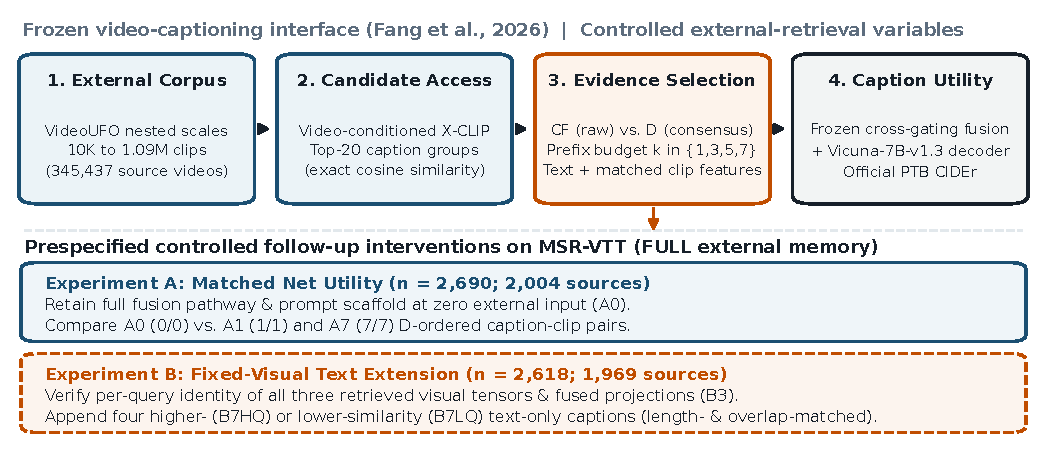
\includegraphics[width=0.96\linewidth]{figures/fig1_framework.pdf}
\caption{Unified diagnostic framework. Corpus scale governs the searchable VideoUFO pool, X-CLIP provides top-20 candidate access, ordering and budget control the text--visual pairs supplied to the frozen captioner, and official PTB CIDEr evaluates caption utility. Experiment A holds the fusion pathway active to compare zero, one, and seven external pairs; Experiment B holds all three retrieved visual tensors and intermediate fused representations identical per query while appending four length- and overlap-matched captions.}
\label{fig:fig1_framework}
\end{figure}

\section{Experimental Setup}
\subsection{Benchmarks, checkpoints, and validation decoder repair}
We evaluate on two standard video-captioning benchmarks using the inherited dataset splits and frozen checkpoints from \\citet{Fang2026EVCap}. \textbf{MSR-VTT} \\citep{Xu2016MSRVTT} comprises 6,513 training, 497 validation (\texttt{val497}), and 2,990 test videos (20 references per video). Because 300 test videos were inspected during early development, we exclude them from formal test inference, yielding a 2,690-query pilot-excluded evaluation cohort (\texttt{test2690}). \textbf{MSVD} \\citep{Chen2011MSVD,Fang2026EVCap} follows the 1,200/100/670 train/validation/test split and is evaluated using the external settings carried over from MSR-VTT without MSVD-specific budget tuning. Because both benchmarks were analyzed prior to designing the follow-up interventions---and pilot exclusion does not guarantee complete source disjointness from development---we treat the historical test budget sweeps as frozen retrospective evaluations and report the follow-up interventions explicitly as prespecified experiments conducted on previously analyzed benchmark material.

A critical architectural asymmetry distinguishes the two inherited checkpoints: \textbf{the MSR-VTT checkpoint was trained with a budget of seven examples, whereas the MSVD checkpoint was trained with a budget of three} \\citep{Fang2026EVCap}. Consequently, moving from $k=1$ to $k=3$ stays within MSVD's original training operating range, whereas $k=5$ and $k=7$ test extrapolation beyond it. All inference runs use beam width 5, random seed 42, deterministic caption-to-clip mapping, and identical prompt templates within each benchmark, with query-retrieval frames and retrieved-video fusion frames extracted via their respective whole-video sampling protocols (Supplementary Materials S2).

\textbf{Validation video-decoder disclosure:} Earlier raw-video evaluation runs on MSR-VTT \texttt{val497} and a 150-query leave-one-out subset (\texttt{val150}) were affected by a degenerate evaluation decode window that collapsed raw video inputs to repeated early frames (Supplementary Materials S9). In contrast, \texttt{test2690}, MSVD test670, and all X-CLIP retrieval embeddings used pre-extracted whole-video frame paths and were never affected. Repairing the raw-video decode window restored full whole-video decoding across all 48 scale-grid conditions and all validation mechanism diagnostics (modality factorial, matched in-domain control, Oracle selection, prompt order, tail swaps, and \texttt{val150} leave-one-out). Every validation number reported in this paper comes exclusively from repaired whole-video outputs; earlier pre-fix validation claims that lost statistical support after repair (including strong text-overload and domain-reversal claims) are permanently excluded.

\subsection{Metrics and retrospective inference}
Official \textbf{CIDEr} \\citep{Vedantam2015CIDEr}, computed with the Stanford PTB tokenizer and frozen COCO-style evaluator and multiplied by 100 (expressed in \textbf{points}), serves as our primary outcome for both absolute means and paired differences. Within any scored split, all compared systems share identical reference documents and reference document frequencies. To test sensitivity to fixed corpus IDF weighting, we also re-estimated document frequencies inside 999 source-cluster bootstrap resamples for the two key Oracle contrasts. Secondary metrics include BLEU-1, BLEU-4, METEOR, ROUGE-L, and SPICE \\citep{Papineni2002BLEU,Banerjee2005METEOR,Lin2004ROUGE,Anderson2016SPICE}. For descriptive output behavior, we compute mean word count and generated trigram match rates against both the union of supplied captions and the fixed top-1 retrieved caption (without crossing caption boundaries).

Paired contrasts are formed per query, and uncertainty is quantified using 10,000 paired bootstrap resamples and 10,000 two-sided sign-flip permutations with a fixed seed. Because multiple clips can originate from the same YouTube video, our primary inference resamples and sign-flips \textbf{source clusters} as intact units (361 sources in \texttt{val497}, 2,004 in \texttt{test2690}, 522 in MSVD, and 137 in \texttt{val150}), weighting resampled means by sampled clip counts. All reported 95\% confidence intervals are pointwise rather than simultaneous intervals and condition on the fixed retrieval corpora. For retrospective benchmark and diagnostic families, we control the false discovery rate via Benjamini--Hochberg (BH) separately across the 72-contrast validation grid, the 4-contrast Oracle family (with a combined 76-test sensitivity check), the benchmark test families (7 contrasts in MSR-VTT; 6 in MSVD), and exploratory diagnostic families (47 cross-scale/aggregate, 18 mechanism, and 8 leave-one-out contrasts).

\subsection{Prespecified controlled follow-up interventions}
To answer RQ2 and RQ3 directly, we froze two intervention protocols, exact input fingerprints, eligibility rules, endpoints, and statistical plans prior to running six new inference arms on the FULL external memory with the MSR-VTT checkpoint. All six arms generated outputs on the full 2,990 test queries for end-to-end trace verification, while formal inference strictly excluded the 300 development pilot queries.

\textbf{Experiment A (Matched zero-evidence net utility; \emph{n} = 2,690 queries, 2,004 sources):} Arm \textbf{A0} receives empty external caption and similarity lists, loads zero retrieved video features, and supplies an all-zero $1 \times 32 \times 768$ external aggregate tensor to the cross-attention keys and values---while keeping the query video, prompt scaffold, cross-attention, learned gating layers, linear projections, and Vicuna-7B decoder active. A0 therefore isolates the operating point of the trained retrieval-augmented architecture at zero external evidence; it is neither a separately retrained no-retrieval baseline nor an architecture with fusion disabled. Arms \textbf{A1} and \textbf{A7} supply the first one and seven D-ordered caption--clip pairs. Per-query traces verify parity of query frames, Q-Former inputs, query visual projections, module states, and encoder RNG fingerprints across all three arms. Prespecified primary contrasts are \textbf{A1 $-$ A0} and \textbf{A7 $-$ A0}; \textbf{A1 $-$ A7} is strictly descriptive.

\textbf{Experiment B (Fixed-visual textual extension; \emph{n} = 2,618 eligible queries, 1,969 sources):} Arm \textbf{B3} supplies the first three D-ordered caption--clip pairs. Arms \textbf{B7HQ} and \textbf{B7LQ} retain the exact same three head captions and the exact same three retrieved visual inputs, appending four text-only captions selected from the eight highest-scoring (HQ) or eight lowest-scoring (LQ) remaining candidates in the raw X-CLIP top-20 pool. Prespecified matching constraints require each appended quartet to draw from four distinct representative sources disjoint from the head, separate the HQ and LQ quartets by at least 0.005 in mean raw X-CLIP similarity, and minimize normalized imbalances in total word count, word-set Jaccard overlap with the head, and internal Jaccard overlap within the quartet, without ever consulting references or generated outputs. Here HQ and LQ denote \textbf{relative X-CLIP similarity bands}, not human-verified semantic quality labels.

Of the 2,690 pilot-excluded queries, \textbf{2,618} satisfied all eligibility constraints (the remaining 72 queries and 300 pilots received the B3 head alone across all three arms). Across all 2,990 queries, runtime traces verified exact per-query identity of the three retrieved feature tensors, similarity weights, visual aggregate, attention keys and values, gate inputs, and visual projections across B3, B7HQ, and B7LQ (Supplementary Table S6). Only the appended text captions and resulting prompt tokens varied. Prespecified primary contrasts are \textbf{B7HQ $-$ B3}, \textbf{B7LQ $-$ B3}, and \textbf{B7HQ $-$ B7LQ}.

\textbf{Follow-up statistical plan:} Official PTB CIDEr fits reference document frequencies separately on each scored cohort (shared by all arms within A or within B), so absolute CIDEr means are not directly comparable across A and B. Inference uses 10,000 source-cluster bootstrap resamples and 10,000 two-sided source-level sign flips (seed 20261125). Familywise error is controlled at $\alpha = .05$ via \textbf{Holm adjustment} both within each experiment (two tests in A; three tests in B) and jointly across \textbf{all five planned contrasts} for cross-experiment claims. We additionally prespecified a \textbf{practical clarity criterion}: an effect is deemed practically clear only if it passes adjusted significance \emph{and} its pointwise 95\% confidence interval lies wholly above +1.0 or wholly below $-$1.0 CIDEr point. Non-discovery does not establish equivalence.

\section{Results: Corpus Scale, Access, and Joint Evidence Budgets}
\subsection{Nested corpus scale and joint budget grid (RQ1)}
Table 1 summarizes official PTB CIDEr across the six nested VideoUFO scales, two candidate orderings, and four joint text--visual budgets on the repaired 497-query MSR-VTT validation split. Holding budget fixed, expanding the external corpus from 10K to 1.09M clips produces no consistent monotonic gain in caption utility. At $k=3$, for instance, moving from 10K to FULL shifts CIDEr by +0.83 points under D (95\% source-cluster CI [$-$1.26, +2.88]) and by $-$1.25 points under CF ([$-$3.42, +0.90]). Across the retrospective 72-contrast validation grid family (four budget contrasts per scale--ordering cell plus four CF--D contrasts per scale), zero contrasts survive BH adjustment at FDR 0.05 (minimum query-level BH $q = 0.1649$ in the PTB reanalysis; $0.1589$ on archived printed $p$-values).

\begin{table}[t]
\centering
\footnotesize
\caption{Repaired MSR-VTT validation CIDEr (official PTB points; \emph{n} = 497, 361 sources) across six nested VideoUFO clip scales, two candidate orderings (CF raw similarity, D full-caption consensus), and four paired text--visual budgets.}
\label{tab:1}
\resizebox{\linewidth}{!}{%
\begin{tabular}{lrrrrrrrr}
\toprule
\textbf{Corpus scale (clips)} & \textbf{CF1} & \textbf{CF3} & \textbf{CF5} & \textbf{CF7} & \textbf{D1} & \textbf{D3} & \textbf{D5} & \textbf{D7} \\
\midrule
10K (10,000) & 70.43 & 70.13 & 69.30 & 68.73 & 69.21 & 67.80 & 67.67 & 67.33 \\
50K (50,000) & 69.98 & 68.47 & 68.08 & 67.09 & 68.89 & 67.84 & 66.80 & 66.12 \\
100K (100,000) & 69.89 & 70.10 & 69.32 & 67.57 & 69.61 & 68.68 & 66.69 & 66.15 \\
250K (250,000) & 70.50 & 69.09 & 67.80 & 68.77 & 70.29 & 69.29 & 68.75 & 66.99 \\
500K (500,000) & 70.50 & 68.87 & 68.89 & 67.23 & 70.59 & 70.08 & 68.25 & 67.62 \\
FULL (1,091,712) & 71.17 & 68.88 & 68.84 & 67.95 & 69.97 & 68.63 & 67.31 & 67.22 \\
\bottomrule
\end{tabular}%
}
\end{table}

Descriptively, the budget pattern is strikingly one-sided: $k=1$ achieves the highest observed mean in 11 of the 12 scale--ordering cells, whereas $k=7$ is highest in none. In addition, raw X-CLIP similarity (CF) matches or slightly exceeds full-caption consensus reranking (D) in most FULL and small-budget cells (e.g., FULL CF1 71.17 vs. D1 69.97), indicating that our consensus approximation does not confer a consistent descriptive advantage over raw retrieval on this machine-captioned external memory. Averaging $k=3$ minus $k=7$ across all 12 cells per query yields an exploratory aggregate of +1.59 CIDEr points (95\% source-cluster CI [+0.23, +2.97]; nominal \emph{p} = .0214; exploratory 47-test $q \approx .503$), while the 10K-to-FULL three-way interaction is imprecisely estimated at $-$1.41 ([$-$5.16, +2.39]). Formal evidence for the budget gradient therefore comes from the larger benchmark test cohorts in Section 5.3.

\subsection{Divergence between retrieval access and generation utility}
Figure 2 directly aligns retrieval-side access against downstream generation utility on the same 497 validation queries at fixed budget $k=3$. Expanding the memory from 10K to FULL replaces the selected top-one clip list on 494 of 497 queries in CF and 495 of 497 in D, driving a steady, monotonic increase in mean selected top-one X-CLIP similarity (+0.0259 for CF and +0.0319 for D; where D reports the original X-CLIP similarity of its consensus-selected candidate). The supplementary candidate-only D7 best-caption reference-overlap proxy likewise rises across the scale endpoints from 13.61 to 18.35 points.

Yet this substantial improvement in candidate access fails to translate into reliable caption gains. At the query level, rank correlations between selected-similarity change and generation CIDEr change from 10K to FULL are essentially zero ($\rho = .011$ for CF; $\rho = .007$ for D), and every scale-versus-10K generation interval crosses zero (Figure 2b). Improving retrieval similarity by expanding the corpus is therefore insufficient to predict downstream generation returns in this frozen interface.

\begin{figure}[t]
\centering
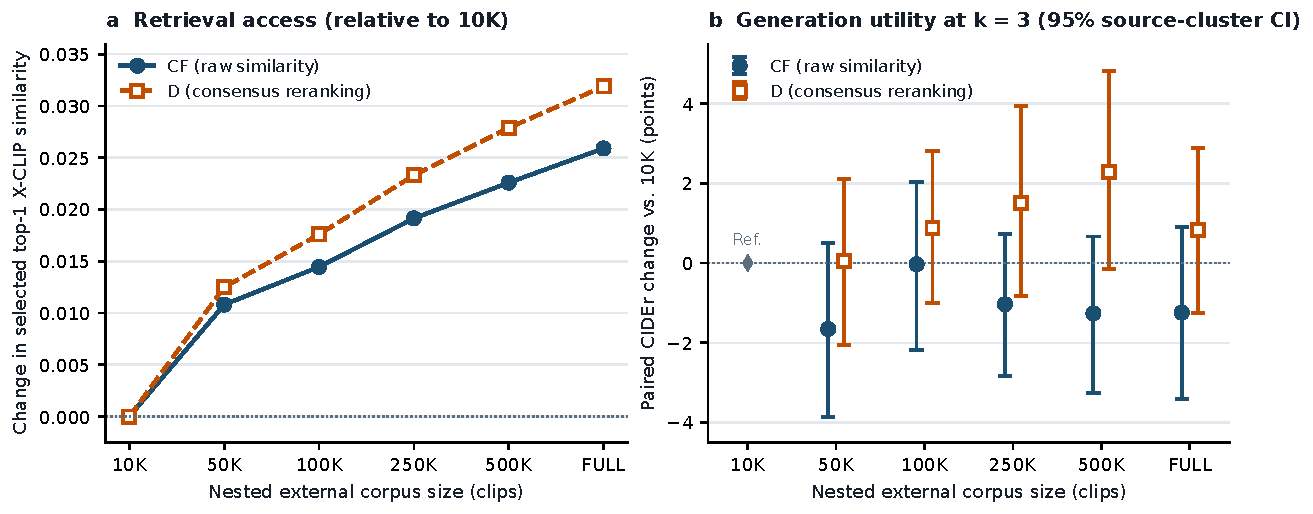
\includegraphics[width=0.96\linewidth]{figures/fig2_access.pdf}
\caption{Retrieval access versus downstream caption utility at fixed budget $k=3$ on repaired MSR-VTT validation (\emph{n} = 497; 361 sources). (a) Mean change in selected top-one X-CLIP cosine similarity relative to 10K increases monotonically for both CF (raw) and D (consensus). (b) Paired CIDEr changes relative to 10K (pointwise 95\% source-cluster CIs) fluctuate in both directions and span zero across all scales.}
\label{fig:fig2_access}
\end{figure}

\subsection{Cross-benchmark joint budget response on MSR-VTT and MSVD}
On both frozen test benchmarks, external retrieval exhibits a monotonic negative gradient across joint budgets from $k=1$ to $k=7$ (Tables 2--3; Figure 3; full benchmark families in Supplementary Table S2). On pilot-excluded MSR-VTT (\emph{n} = 2,690; 2,004 sources), CIDEr declines from 71.21 (D1) to 70.08 (D3), 69.48 (D5), and 68.27 (D7). Both \textbf{D1 $-$ D3} (+1.13 points, 95\% source-cluster CI [+0.35, +1.94], BH \emph{q} = .0083) and \textbf{D3 $-$ D7} (+1.80 points, [+0.86, +2.76], \emph{q} = .0007) survive source-cluster BH adjustment, yielding a cumulative D1 $-$ D7 advantage of +2.93 points ([+1.83, +4.06], \emph{q} = .0007). Notably, this decline occurs on a checkpoint trained at $k=7$, so degradation at seven external pairs cannot be dismissed as unseen prompt length. The archived in-domain MSR-VTT comparator remains strongest at 73.09 CIDEr (+1.88 over D1, [+0.77, +2.96], \emph{q} = .0019).

\begin{table}[t]
\centering
\footnotesize
\caption{Frozen test-set PTB CIDEr means on pilot-excluded MSR-VTT (\emph{n} = 2,690) and MSVD (\emph{n} = 670) using the FULL external VideoUFO memory. The MSR-VTT in-domain comparator uses training captions; separately attributed MSVD in-domain references (published 158.1; archival reproduction 158.32) are documented in Supplementary Materials S3.}
\label{tab:2}
\resizebox{\linewidth}{!}{%
\begin{tabular}{lrrrrrr}
\toprule
\textbf{Benchmark} & \textbf{D1} & \textbf{D3} & \textbf{D5} & \textbf{D7} & \textbf{Adaptive} & \textbf{In-domain} \\
\midrule
MSR-VTT (\texttt{test2690}) & 71.21 & 70.08 & 69.48 & 68.27 & 70.67 & 73.09 \\
MSVD (\texttt{test670}) & 156.39 & 151.45 & 144.39 & 141.59 & 151.94 & --- \\
\bottomrule
\end{tabular}%
}
\end{table}

\begin{table}[t]
\centering
\small
\caption{Selected paired test-set contrasts (PTB CIDEr points) with pointwise 95\% source-cluster bootstrap CIs, two-sided sign-flip \emph{p}-values, and within-benchmark BH-adjusted \emph{q}-values (7 contrasts in MSR-VTT; 6 in MSVD; complete tables in Supplementary Table S2).}
\label{tab:3}
\resizebox{\linewidth}{!}{%
\begin{tabular}{llrrrr}
\toprule
\textbf{Benchmark} & \textbf{Contrast} & \textbf{Effect} & \textbf{95\% source-cluster CI} & \textbf{Source \emph{p}} & \textbf{Source BH \emph{q}} \\
\midrule
MSR-VTT & D1 $-$ D3 & +1.13 & [+0.35, +1.94] & .0059 & .0083 \\
MSR-VTT & D3 $-$ D7 & +1.80 & [+0.86, +2.76] & .0002 & .0007 \\
MSR-VTT & D1 $-$ D7 & +2.93 & [+1.83, +4.06] & .0001 & .0007 \\
MSR-VTT & Adaptive $-$ D1 & $-$0.54 & [$-$1.20, +0.10] & .1006 & .1006 \\
MSVD & D1 $-$ D3 & +4.94 & [+1.50, +8.39] & .0046 & .0069 \\
MSVD & D3 $-$ D7 & +9.86 & [+5.49, +15.05] & .0001 & .0003 \\
MSVD & D1 $-$ D7 & +14.80 & [+9.92, +19.97] & .0001 & .0003 \\
MSVD & Adaptive $-$ D1 & $-$4.46 & [$-$7.68, $-$1.47] & .0030 & .0060 \\
\bottomrule
\end{tabular}%
}
\end{table}

MSVD (\emph{n} = 670; 522 sources) reproduces the downward gradient: 156.39 (D1), 151.45 (D3), 144.39 (D5), and 141.59 (D7). Crucially, interpreting MSVD requires separating two regimes. Within the inherited checkpoint's 3-context operating range, \textbf{D1 $-$ D3} is +4.94 points ([+1.50, +8.39], \emph{q} = .0069), confirming that external-budget degradation transfers to a second benchmark without exceeding the training count. The larger drop from D3 to D7 (+9.86 points, [+5.49, +15.05], \emph{q} = .0003) extends beyond MSVD's 3-context training budget without a matched MSVD in-domain budget sweep and should be read as an extrapolation regime rather than an unconfounded measure of external overload.

The bounded similarity-gap Adaptive comparator yields intermediate CIDEr means (70.67 on MSR-VTT; 151.94 on MSVD). It trails fixed D1 by $-$0.54 points on MSR-VTT (CI crosses zero, \emph{q} = .1006) and significantly trails fixed D1 by $-$4.46 points on MSVD ([$-$7.68, $-$1.47], \emph{q} = .0060). Moreover, because its routing rule was chosen using earlier validation data prior to the decoder repair, its favorable margins over larger budgets do not validate that earlier selection step. Small fixed budgets therefore serve as the stronger and simpler operational reference.

\begin{figure}[t]
\centering
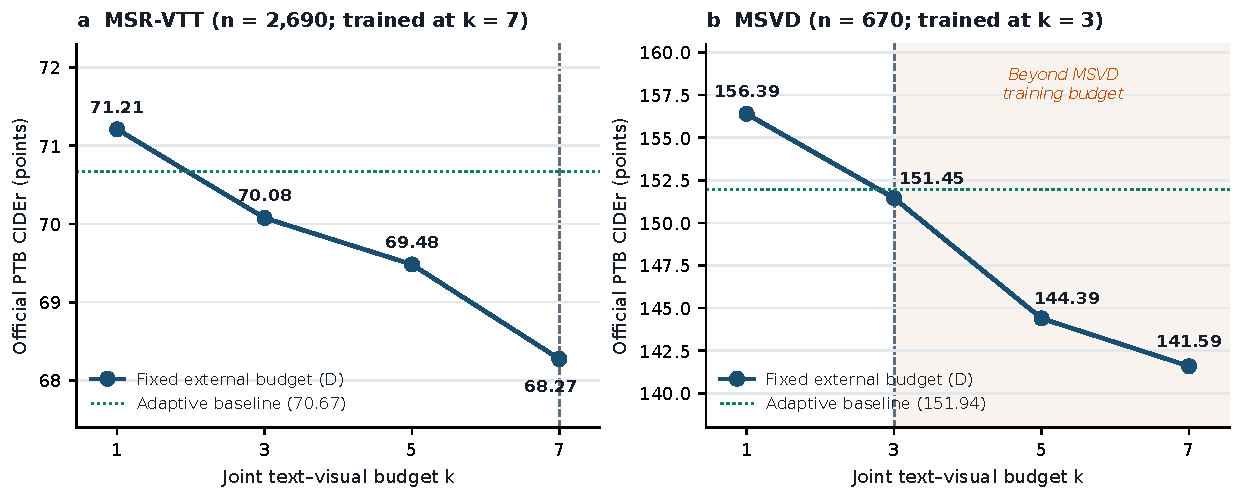
\includegraphics[width=0.96\linewidth]{figures/fig3_budget.pdf}
\caption{External D-ordering CIDEr curves across joint text--visual budgets on (a) pilot-excluded MSR-VTT (\emph{n} = 2,690; trained at $k=7$) and (b) MSVD (\emph{n} = 670; trained at $k=3$). Vertical dashed lines denote each checkpoint's inherited training budget; shading in (b) marks extrapolation beyond MSVD's 3-context training regime. Horizontal dotted lines mark the bounded Adaptive comparator. Each panel uses its benchmark-specific vertical scale and reference corpus.}
\label{fig:fig3_budget}
\end{figure}

\section{Controlled Follow-up Experiments: Net Utility and Fixed-Visual Text Extensions}
While Section 5 establishes that smaller joint budgets outperform larger ones, positive-budget curves leave two fundamental questions open: whether external retrieval provides a net gain over zero external evidence (RQ2), and whether appending textual captions alone reproduces the large-budget loss when retrieved visual inputs are held strictly identical (RQ3). Tables 4--5 and Figures 4--5 present the formal source-cluster results for our two prespecified MSR-VTT interventions.

\subsection{Experiment A: Matched zero-evidence net utility (RQ2)}
Holding the MSR-VTT checkpoint, query video, prompt scaffold, cross-gating fusion layers, and decoding fixed, the matched zero-evidence control \textbf{A0} scores \textbf{69.81 CIDEr points} (Table 4; Figure 4a). Supplying one external caption--clip pair (\textbf{A1}) raises CIDEr to \textbf{71.21}, whereas supplying seven pairs (\textbf{A7}) lowers CIDEr to \textbf{68.27}.

Formal paired source-cluster inference (Table 5; Figure 5) establishes that \textbf{A1 $-$ A0 = +1.40 CIDEr points} (95\% pointwise source-cluster CI [+0.45, +2.36]; raw \emph{p} = .0033). This gain survives Holm adjustment both within Experiment A (family Holm \emph{p} = .0066) and across \textbf{all five prespecified follow-up tests} (five-test Holm \emph{p} = .0165). It represents the strongest new empirical finding of the study: in this trained retrieval-augmented system, one external caption--clip pair from a million-clip machine-described memory delivers a statistically supported net utility gain over operating the same fusion-enabled system with empty external input.

By contrast, evidence for net harm at seven pairs is weaker and multiplicity-dependent. \textbf{A7 $-$ A0 = $-$1.54 points} (95\% CI [$-$2.94, $-$0.18]; raw \emph{p} = .0271) passes Holm correction within the two-test A family (family Holm \emph{p} = .0271) but does \textbf{not} meet the .05 threshold under joint five-test Holm adjustment (\emph{p} = .0813). Furthermore, neither A1 $-$ A0 nor A7 $-$ A0 clears the prespecified practical clarity criterion: both pointwise 95\% CIs include magnitudes smaller than 1.0 CIDEr point (Figure 5). The descriptive A1 $-$ A7 difference is +2.93 points. On all 2,990 test queries, the newly executed A1 and A7 predictions match the archived D1 and D7 output records identically, confirming exact endpoint reproducibility; we accordingly treat those matching endpoints as a verification check rather than an independent second sample.

\begin{table}[t]
\centering
\small
\caption{Cohort-specific PTB CIDEr means and observed wrapped prompt lengths (including visual token positions) for Experiments A and B on MSR-VTT (FULL external memory). Because reference IDF is fitted separately within each scored cohort, absolute means should be compared strictly within Experiment A or within Experiment B.}
\label{tab:4}
\resizebox{\linewidth}{!}{%
\begin{tabular}{llrrrr}
\toprule
\textbf{Experiment} & \textbf{Arm} & \textbf{Text / retrieved visuals} & \textbf{Scored queries (sources)} & \textbf{Cohort CIDEr} & \textbf{Mean prompt length (median)} \\
\midrule
A & A0 & 0 / 0 & 2,690 (2,004) & 69.81 & --- \\
A & A1 & 1 / 1 & 2,690 (2,004) & 71.21 & --- \\
A & A7 & 7 / 7 & 2,690 (2,004) & 68.27 & --- \\
B & B3 & 3 / 3 & 2,618 (1,969) & 69.88 & 150.69 (148) \\
B & B7HQ & 7 / 3 & 2,618 (1,969) & 68.62 & 226.86 (224) \\
B & B7LQ & 7 / 3 & 2,618 (1,969) & 68.75 & 226.38 (223) \\
\bottomrule
\end{tabular}%
}
\end{table}

\begin{figure}[t]
\centering
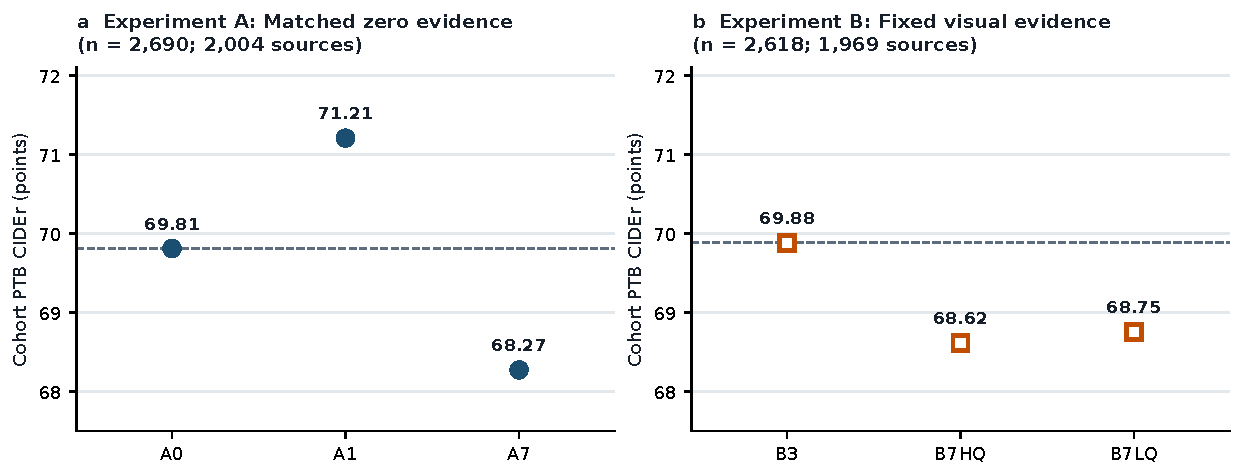
\includegraphics[width=0.96\linewidth]{figures/fig4_followups.pdf}
\caption{Cohort-specific PTB CIDEr means for the two prespecified interventions on MSR-VTT. (a) Experiment A compares empty external input (A0, dashed reference line) against one (A1) and seven (A7) caption--clip pairs with the fusion pathway active. (b) Experiment B holds all three retrieved visual tensors identical to B3 (dashed reference line) and appends four higher-similarity (B7HQ) or lower-similarity (B7LQ) captions. Comparisons are strictly within panel because reference IDF is cohort-specific.}
\label{fig:fig4_followups}
\end{figure}

\subsection{Experiment B: Fixed-visual text extensions (RQ3)}
On the 2,618 eligible queries (1,969 sources), runtime traces verified exact per-query identity of the three retrieved visual feature tensors, similarity weights, fused aggregate, attention keys and values, gating inputs, and visual projections across B3, B7HQ, and B7LQ (Supplementary Table S6). Visual variation is therefore eliminated as a confound inside Experiment B.

The baseline three-pair head \textbf{B3} scores \textbf{69.88 CIDEr points}. Appending four higher-similarity captions (\textbf{B7HQ}) lowers the mean to \textbf{68.62}, and appending four lower-similarity captions (\textbf{B7LQ}) lowers it to \textbf{68.75} (Table 4; Figure 4b). Both paired contrasts are negative with pointwise 95\% source-cluster CIs excluding zero: \textbf{B7HQ $-$ B3 = $-$1.27 points} ([$-$2.34, $-$0.20]; raw \emph{p} = .0191) and \textbf{B7LQ $-$ B3 = $-$1.13 points} ([$-$2.15, $-$0.14]; raw \emph{p} = .0306). Crucially, however, \textbf{neither extension survives Holm correction within the three-test B family} (family Holm \emph{p} = .0573 and .0612; five-test Holm \emph{p} = .0764 and .0813; Table 5).

The direct equal-count contrast between similarity bands is inconclusive: \textbf{B7HQ $-$ B7LQ = $-$0.14 points} (95\% CI [$-$1.05, +0.80]; raw, family Holm, and five-test Holm \emph{p} = .7698). Because the interval spans zero and extends past $-$1.0, the data establish neither superiority of the higher-similarity band nor statistical equivalence between bands. Matching quality between B7HQ and B7LQ was tight (Supplementary Table S4): mean wrapped prompt lengths were 226.86 versus 226.38 tokens (mean difference +0.48; median absolute difference 3; compared against 150.69 in B3), mean absolute quartet word imbalance was 0.35 words, head-overlap and internal-overlap Jaccard imbalances averaged 0.0085 and 0.0074, and the mean raw X-CLIP similarity separation between bands was \textbf{0.00835} (range 0.00500--0.02606). Together, these findings offer directional---but statistically unconfirmed---evidence of a cost from appending these matched text quartets, while showing that a narrow X-CLIP similarity gap does not reliably separate their utility.

\begin{table}[t]
\centering
\footnotesize
\caption{All five prespecified paired contrasts from Experiments A and B (PTB CIDEr points), reporting pointwise 95\% source-cluster bootstrap CIs, two-sided source-level sign-flip \emph{p}-values, within-family Holm \emph{p}-values, five-test Holm \emph{p}-values, and whether each contrast meets the prespecified $\pm$1.0-point practical clarity rule.}
\label{tab:5}
\resizebox{\linewidth}{!}{%
\begin{tabular}{llrrrrrrl}
\toprule
\textbf{Family} & \textbf{Contrast} & \textbf{Queries (sources)} & \textbf{Effect} & \textbf{95\% source-cluster CI} & \textbf{Raw \emph{p}} & \textbf{Family Holm \emph{p}} & \textbf{Five-test Holm \emph{p}} & \textbf{Clear practical effect ($\pm$1 pt)} \\
\midrule
A & A1 $-$ A0 & 2,690 (2,004) & +1.40 & [+0.45, +2.36] & .0033 & \textbf{.0066} & \textbf{.0165} & No \\
A & A7 $-$ A0 & 2,690 (2,004) & $-$1.54 & [$-$2.94, $-$0.18] & .0271 & \textbf{.0271} & .0813 & No \\
B & B7HQ $-$ B3 & 2,618 (1,969) & $-$1.27 & [$-$2.34, $-$0.20] & .0191 & .0573 & .0764 & No \\
B & B7LQ $-$ B3 & 2,618 (1,969) & $-$1.13 & [$-$2.15, $-$0.14] & .0306 & .0612 & .0813 & No \\
B & B7HQ $-$ B7LQ & 2,618 (1,969) & $-$0.14 & [$-$1.05, +0.80] & .7698 & .7698 & .7698 & No \\
\bottomrule
\end{tabular}%
}
\end{table}

\begin{figure}[t]
\centering
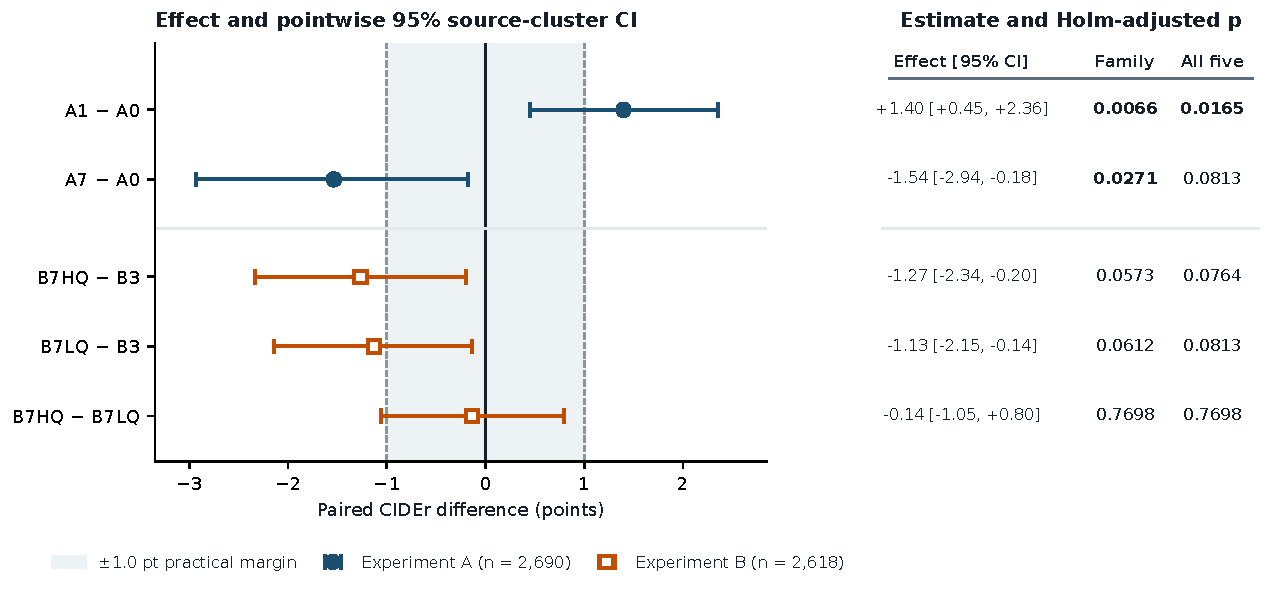
\includegraphics[width=0.96\linewidth]{figures/fig5_forest.pdf}
\caption{Forest plot of all five prespecified contrasts in Experiments A and B. Error bars show pointwise 95\% source-cluster bootstrap CIs (not simultaneous intervals); the shaded band marks the prespecified $\pm$1.0 CIDEr point practical margin. Right columns list exact estimates and Holm-adjusted \emph{p}-values within each family and across all five tests (bold indicates adjusted \emph{p} < .05). No interval lies wholly outside the shaded practical margin.}
\label{fig:fig5_forest}
\end{figure}

\section{Selection Headroom, Alternative Mechanisms, and Output Behaviour}
To contextualize Experiments A and B within the broader diagnostic evidence chain, we summarize our repaired MSR-VTT validation analyses (\texttt{val497} and \texttt{val150}) alongside descriptive output-length and lexical-reuse patterns on the test benchmarks.

\subsection{Reference-guided selection headroom}
Reordering the FULL top-20 validation pool with reference-guided unigram TF-IDF compatibility (Section 3.3) probes whether better candidate selection exists inside the retrieved pool (Table 6). At $k=3$, \textbf{Oracle3 $-$ D3 = +3.04 CIDEr points} (95\% source-cluster CI [+0.85, +5.27]; BH \emph{q} = .0146 within the 4-test Oracle family), confirming meaningful selection headroom. Yet extending the reference-guided prefix from three to seven pairs still reduces performance: \textbf{Oracle7 $-$ Oracle3 = $-$2.73 points} ([$-$4.72, $-$0.80]; \emph{q} = .0146). Re-estimating reference document frequencies inside 999 source-cluster bootstrap resamples yields closely aligned intervals ([+0.78, +5.30] and [$-$4.87, $-$0.94]). At $k=1$ and $k=7$, Oracle gains over D (+1.67 and +1.72 points) have intervals crossing zero (\emph{q} = .1531). Importantly, this diagnostic shows clear sensitivity to multiplicity scope: combining the four Oracle tests with the 72-test validation grid yields query-level BH \emph{q} = .1368 for both Oracle3 $-$ D3 and Oracle7 $-$ Oracle3.

\begin{table}[t]
\centering
\small
\caption{Reference-guided Oracle contrasts on repaired MSR-VTT validation (\emph{n} = 497; 361 sources) with pointwise 95\% source-cluster CIs and BH adjustment within the four-contrast Oracle family.}
\label{tab:6}
\resizebox{\linewidth}{!}{%
\begin{tabular}{lrrrr}
\toprule
\textbf{Contrast} & \textbf{Effect (CIDEr pts)} & \textbf{95\% source-cluster CI} & \textbf{Source \emph{p}} & \textbf{Source BH \emph{q}} \\
\midrule
Oracle1 $-$ D1 & +1.67 & [$-$0.50, +3.78] & .1282 & .1531 \\
Oracle3 $-$ D3 & +3.04 & [+0.85, +5.27] & .0073 & .0146 \\
Oracle7 $-$ D7 & +1.72 & [$-$0.62, +4.08] & .1531 & .1531 \\
Oracle7 $-$ Oracle3 & $-$2.73 & [$-$4.72, $-$0.80] & .0068 & .0146 \\
\bottomrule
\end{tabular}%
}
\end{table}

Furthermore, Oracle7 $-$ Oracle3 cannot isolate pure textual integration overload. By construction, individual reference compatibility declines smoothly down the ranking, averaging 0.1380 at ranks 1--3 versus 0.1031 at ranks 4--7 (Supplementary Materials S4). Across queries, the rank correlation between this head-to-tail compatibility drop and Oracle3 $-$ Oracle7 CIDEr loss is negligible ($\rho = .046$, 95\% source-cluster CI [$-$.044, +.131], with roughly 60\% tied query effects). Because extending the Oracle prefix simultaneously alters candidate count, candidate compatibility, and the visual tensors entering fusion, the Oracle intervention establishes selection headroom and a cost of extending one feasible prefix without isolating text count alone.

\subsection{Repaired validation modality, source, order, tail, and removal controls}
Following the raw-video decoder repair (Section 4.1), none of the 18 validation mechanism contrasts or 8 \texttt{val150} leave-one-out contrasts survive BH correction (complete estimates in Supplementary Table S3):

\begin{itemize}
\item \textbf{Text-by-visual factorial (\emph{n} = 497):} Crossing $T \in \{3, 7\}$ with $V \in \{3, 7\}$ yields a textual main effect of $-$1.37 CIDEr points (95\% source-cluster CI [$-$4.10, +1.26]; \emph{p} = .3154), a tightly bounded near-zero visual main effect of $-$0.04 ([$-$0.42, +0.35]; \emph{p} = .8529), and an interaction of +0.16 ([$-$0.60, +0.94]; \emph{p} = .7003). While the compact 32-token visual aggregation shows minimal sensitivity to $V$ here, the wide textual interval motivated the larger-cohort fixed-visual test in Experiment B.
\item \textbf{Matched in-domain control (\emph{n} = 497):} Re-extracting MSR-VTT training video features under the identical pipeline gives an in-domain D3 $-$ D7 difference of $-$1.34 ([$-$3.59, +0.92]) versus +1.41 ([$-$1.21, +4.17]) for FULL external retrieval, yielding an imprecisely estimated source-by-budget difference in differences of +2.74 ([$-$0.76, +6.29]; \emph{p} = .1322). This directional contrast neither confirms a formal interaction nor separates domain alignment from corpus size, annotation style, or training distribution.
\item \textbf{Prompt order, tail quality, and leave-one-out (\emph{n} = 497 / 150):} Reversing D7 prompt order ($-$0.24, [$-$2.08, +1.67]) or placing the top three captions last (+0.02, [$-$1.76, +1.92]) centers near zero. Replacing positions 4--7 with reference-compatible captions (GoodTail, $-$0.56, [$-$3.23, +2.04]) fails to reproduce pre-fix gains; HardWrong ($-$1.45, [$-$3.55, +0.66]) and its direct contrast against EasyWrong ($-$1.08, [$-$3.44, +1.22]) remain inconclusive. Removing individual items on \texttt{val150} yields imprecise per-rank estimates (rank 1: +1.97 [$-$1.04, +5.11]; rank 7: $-$1.51 [$-$5.28, +1.97]; head minus tail: +1.06 [$-$0.18, +2.40]), showing no reliable concentration of harm in specific ranks.
\end{itemize}
\subsection{Output length, lexical reuse, and metric divergence}
Descriptive inspection of generated test captions clarifies how output text changes as joint budgets expand (Supplementary Table S7). On MSR-VTT \texttt{test2690}, mean caption length rises monotonically from 7.92 words at D1 to 8.75 words at D7, while the fraction of generated trigrams appearing in the union of supplied captions more than doubles from 0.142 to 0.334. Even when the matching target is held strictly fixed to the single top-ranked retrieved caption, trigram reuse still increases from 0.142 to 0.190, demonstrating that mere expansion of the matching union cannot explain the entire lexical-reuse increase. On MSVD, mean length rises similarly from 6.77 to 7.61 words. Across both test sets, archived SPICE scores increase modestly at larger budgets even as CIDEr, BLEU, and ROUGE-L decline. Because automatic n-gram and scene-graph metrics emphasize distinct surface properties and provide no independent verification of visual factuality, this descriptive co-movement neither proves that lexical copying causes the CIDEr drop nor establishes semantic improvement.

\section{Discussion}
\subsection{Why larger external memories do not guarantee better captions}
Across six nested VideoUFO scales spanning two orders of magnitude, X-CLIP retrieval access improved substantially---replacing nearly every top-one candidate by FULL scale---yet fixed-budget generation utility fluctuated without a reliable upward trend. Two factors help explain this dissociation in a frozen captioner. First, retrieval similarity scores match broad visual semantics rather than the exact action framing rewarded by benchmark reference descriptions; replacing a 10K candidate with a slightly higher-similarity 1.09M candidate changes lexical phrasing without necessarily improving event accuracy. Second, the consensus reranking approximation (D) showed no consistent descriptive benefit over raw X-CLIP similarity (CF) externally, likely reflecting differences between machine-generated VideoUFO brief captions and clean human benchmark annotations, as well as our full-caption ROUGE-L approximation to Fang et al.'s noun-phrase formulation. Retrieval-side metrics alone are therefore an incomplete deployment criterion for scaled external memories.

\subsection{What the matched zero-evidence control reveals about budget choice}
Without a zero-evidence anchor, observing that D1 outscores D7 on MSR-VTT and MSVD remained fundamentally ambiguous: a smaller positive budget could either capture genuine external value or merely inflict less harm than a larger budget. Experiment A resolves that ambiguity for the tested MSR-VTT checkpoint. Retaining the full fusion architecture at zero external input places A0 (69.81) squarely between A1 (71.21) and A7 (68.27). Single-pair retrieval confers a statistically robust net gain (+1.40, surviving five-test Holm correction), whereas expanding to seven pairs shifts the mean below zero evidence ($-$1.54, supported within the A family but falling short of five-test Holm correction).

This sign reversal illustrates that evidence budgeting is not merely a minor hyperparameter refinement: within the same frozen model and corpus, budget choice determines whether external retrieval helps or moves performance below an empty-evidence baseline. At the same time, discipline over practical magnitude remains necessary---none of the five planned intervals cleared the prespecified $\pm$1.0-point margin---so the benefit of one external pair should be described as a conditional, modest net gain rather than a large universal improvement.

\subsection{Attribution boundaries: why text overload and similarity proxies remain unconfirmed}
Experiment B closes a major methodological gap in multimodal RAG diagnosis by verifying per-query identity of the actual retrieved visual tensors and intermediate fused projections while varying only appended text. Both B7HQ and B7LQ moved mean CIDEr downward relative to B3 ($-$1.27 and $-$1.13 points), aligning directionally with the joint-budget decline without requiring any visual-input change. Nevertheless, neither extension passed B-family Holm adjustment (\emph{p} = .0573 and .0612), and Experiment B cannot decompose A1 $-$ A7, quantify the share of joint-budget loss attributable to text, or establish an internal attention-distraction mechanism.

Similarly, the near-zero contrast between B7HQ and B7LQ ($-$0.14, [$-$1.05, +0.80]) does not prove that candidate relevance is irrelevant to captioning. Matching quartets across word count, head overlap, and internal overlap restricted the raw X-CLIP similarity separation to an average of 0.00835, and raw cosine bands are only noisy proxies for human-judged semantic relevance. Combined with the repaired validation controls---where position, tail-quality, and leave-one-out interventions all remained statistically inconclusive---our findings counsel caution against importing broad "general text overload" narratives from text QA without stronger semantic controls or mechanistic probing.

\subsection{Practical implications for retrieval-augmented captioning evaluation}
For practitioners deploying frozen captioners with large external memories, our evidence points to a three-part evaluation protocol rather than relying on retrieval similarity or positive-budget sweeps alone. Any external-memory system should report: (1) \textbf{candidate access} under the retriever, (2) \textbf{matched net utility} against the same fusion-enabled architecture receiving empty external input, and (3) \textbf{incremental prefix utility} when extending a working budget. In our frozen system, a small fixed budget ($k=1$) provides the most dependable external operating point---outperforming larger budgets and outperforming or matching the bounded similarity-gap adaptive rule---though our results do not identify a single universally optimal budget across queries or architectures.

\section{Limitations}
Several scope boundaries constrain interpretation of our findings:

\begin{itemize}
\item \textbf{Single frozen architecture and external corpus:} Both prespecified follow-ups evaluate one frozen MSR-VTT checkpoint (Video-LLaMA, X-CLIP, Vicuna-7B-v1.3) and one machine-captioned external memory (VideoUFO brief captions). MSVD corroborates the joint-budget decline under a second inherited checkpoint, but lacks matched zero-evidence or fixed-visual follow-ups, and budgets above $k=3$ exceed its training count. Generalization to modern long-context VLMs that concatenate retrieved video tokens directly, or to human-authored external corpora, remains untested.
\item \textbf{Definition of the zero-evidence baseline (A0):} A0 retains retrieval-trained weights, the prompt scaffold, and active fusion modules with zero external tensors. It answers whether external evidence helps this trained retrieval system; it does not predict the performance of a separately trained video-only captioner without retrieval pathways.
\item \textbf{Scope and proxy limits of Experiment B:} Experiment B applies to the 2,618 MSR-VTT queries admitting balanced, separated quartets (excluding 72 unmatched queries) and tests a narrow raw X-CLIP similarity gap (mean 0.00835) without human semantic-relevance annotations. Appending four captions jointly changes count, prompt length (+76 tokens), and lexical content, so B does not isolate a pure token-count effect.
\item \textbf{Corpus coupling, overlap, and retrospective reuse:} Corpus scale, source diversity, and clip-to-source redundancy co-vary along a single nested chain. Exact YouTube source-ID audits confirm zero source overlap with MSR-VTT splits, yet cannot exclude visual near-duplicates or LLM pretraining exposure. Although Experiments A and B were prespecified before new inference, they evaluate previously analyzed MSR-VTT benchmark queries rather than a newly collected unseen test set.
\item \textbf{Statistical and metric boundaries:} Source-cluster bootstrap intervals capture query-sampling uncertainty conditional on the fixed corpus, checkpoint, and decoding configuration; pointwise 95\% intervals do not provide simultaneous coverage or establish statistical equivalence. Reference-guided Oracle selection shares reference text with evaluation CIDEr and belongs to an exploratory diagnostic family. Finally, automatic metrics (CIDEr, BLEU, METEOR, ROUGE-L, SPICE) and trigram reuse cannot substitute for human adjudication of visual grounding and caption factuality.
\end{itemize}
\section{Conclusion}
Expanding an external video-caption memory to over one million clips substantially increased retrieval similarity and candidate turnover in a fixed multimodal captioner without delivering consistent fixed-budget gains in caption quality. Across both MSR-VTT and MSVD test benchmarks, smaller joint evidence budgets reliably outperformed seven retrieved pairs. In a prespecified matched zero-evidence intervention on MSR-VTT, supplying a single external caption--clip pair yielded a conditional net benefit of +1.40 CIDEr points that survived five-test Holm adjustment, whereas seven pairs fell $-$1.54 points below zero evidence with family-level but not five-test multiplicity support. Holding all three retrieved visual tensors and intermediate fused representations strictly identical per query, appending four higher- or lower-similarity captions produced directional declines ($-$1.27 and $-$1.13 points) that did not pass within-family Holm adjustment, with an inconclusive contrast between similarity bands. Practically, external retrieval should be evaluated not by retrieval scores or positive-budget curves alone, but jointly against a matched zero-evidence baseline and incremental prefix extensions. Within this fixed system, a minimal evidence budget offers a reliable operating point while the precise mechanism of large-budget losses remains open.

\section*{Declarations}
\textbf{Author Contributions:} \emph{[TO BE COMPLETED BY AUTHORS --- e.g., Conceptualization, Methodology, Software, Validation, Formal Analysis, Investigation, Writing -- Original Draft, Writing -- Review \& Editing, Supervision.]}

\textbf{Funding:} \emph{[TO BE COMPLETED BY AUTHORS --- Insert grant agencies and grant numbers, or state "This research received no external funding."]}

\textbf{Competing Interests:} \emph{[TO BE COMPLETED BY AUTHORS --- Confirm whether any authors hold financial or non-financial conflicts of interest, and note any shared authorship with \\citet{Fang2026EVCap} per target journal policy.]}

\textbf{Ethics Approval:} This study performs secondary computational analysis on publicly available benchmark video datasets (MSR-VTT, MSVD) and a publicly released video-caption collection (VideoUFO). No human-subjects experiments or new personal data collection were conducted. \emph{[Authors to verify any institutional disclosure required by target journal.]}

\textbf{Data and Code Availability:} MSR-VTT \\citep{Xu2016MSRVTT} and MSVD \\citep{Chen2011MSVD} are established public benchmarks. VideoUFO metadata and brief captions are used under the CC BY 4.0 license declared in its official dataset card \\citep{VideoUFOCard}; raw third-party YouTube videos are not redistributed. Prespecified intervention protocols, integrity receipts, source-cluster contrast tables, figure-generation scripts, and CPU replay scripts are archived in the project repository (\emph{[Repository URL / DOI to be finalized upon acceptance]}).

\textbf{AI-Assisted Writing Disclosure:} \emph{[TO BE COMPLETED BY AUTHORS --- Declare use of large language model assistance for manuscript drafting, structural editing, and formatting in accordance with the target journal's generative-AI policy; all scientific claims, statistical outputs, and citations were verified by the authors against frozen experimental records.]}

\bibliographystyle{plainnat}
\bibliography{UARCap_References}
\end{document}
